\documentclass[11pt,letterpaper]{article}
\usepackage[utf8]{inputenc}
\usepackage{amsmath}
\usepackage{amsfonts}
\usepackage{amssymb}
\usepackage [english] {babel}
\usepackage{graphicx}
\usepackage{tabularx}
\usepackage{booktabs}
\usepackage{apacite}
\usepackage{xspace}
\usepackage{sectsty}
\usepackage{setspace}
\usepackage{textcomp}
\usepackage{hyperref}
 
\sectionfont{\large}

\begin{document}

\begin{center}
{{\huge \textbf{Medición de la Rotación Diferencial del Sol} \\ 
\singlespacing 
{\large \textbf{María Camila Remolina Gutiérrez\\ 
\normalsize 
\texttt{mc.remolina197@uniandes.edu.co}\\
 }}}}
\end{center}

\hrule

\begin{abstract}
El siguiente artículo tiene como objetivo presentar el proyecto: \textit{Medición de la Rotación Diferencial del Sol}. Se busca introducir al tema, y explicar el método a seguir para obtener el resultado deseado. Todo esto, siendo parte del proyecto final del Seminario de Astronomía y Astrofísica de la misma universidad. \\
\end{abstract}

\hrule

\section{Introducción}
El Sol, al igual que diferentes cuerpos celestes como planetas o asteroides, tiene polo norte, polo sur y gira alrededor de un eje. Sin embargo, la velocidad de esta rotación no es constante en toda la superficie debido a que el Sol no es un sólido en totalidad sino que su fotosfera se encuentra en estado plasmático, lo cual ocasiona que el ecuador gire a velocidades mayores que en los polos. 
\\

Esta rotación diferencial tiene como consecuencia que el campo magnético del Sol se enrede alrededor de él mismo, causando dos fenómenos: erupciones solares y manchas solares. Las primeras suceden cuando este campo enredado se revienta y no vuelve a entrar al sol, liberando cantidades enormes de energía. Por otro lado, las manchas solares se producen cuando el campo que se rompió vuelve a entrar a la superficie, produciendo una diferencia de temperatura e intensidad luminosa, que en comparación a la luz total emitida por el sol se ve relativamente oscura.
\\

\hrule

\section{Objetivos}
El objetivo principal del proyecto es poder calcular los diferentes periodos en los que gira la superficie del sol por medio manchas solares con datos experimentales tomados desde el observatorio de la Universidad de los Andes.\\

\hrule

\section{Metodología}

La manera como se llevara a cabo este proyecto se divide en dos etapas: toma de datos y la obtención de resultados.\\

\subsection{Toma de Datos}

Debido a que este proyecto es en gran parte observacional, la toma de datos es una parte fundamental en el proceso. Para esto, de lunes a viernes 2 veces al día (mañana y tarde) se realizan tomas fotográficas al Sol desde el observatorio astronómico de la Universidad de los Andes. Sin embargo, debido a las condiciones climáticas de la ciudad de Bogotá, en repetidas ocasiones no es posible observar al sol en su totalidad; por esta razón, y también para comparar y poder localizar la imagen tomada en la posición correcta, se utilizan las fotografías satelitales que ofrece el Lockheed-Martin Solar and Astrophysics Laboratory (LMSAL) provistas por el Solar Dynamics Obsbervatory (SDO).
\\

\subsection{Obtención de Resultados}

Para el análisis de los datos obtenidos, hay que primero introducir el tema de coordenadas heliográficas, que en otras palabras es dividir el mapa del sol en una rejilla que se asemeja a las latitudes y longitudes de la Tierra.
\\

\begin{figure}[h!]
 \centering
 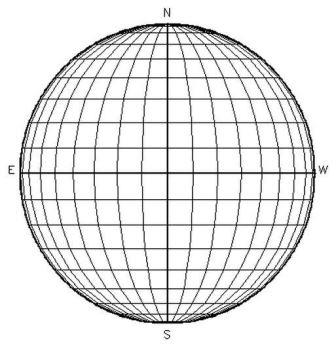
\includegraphics[width=0.7\linewidth]{./grid}
 \caption{Rejilla Solar. \href{http://sohowww.nascom.nasa.gov/explore/lessons/sun_grid.gif}{Obtenido de: $http://sohowww.nascom.nasa.gov/explore/lessons/sun_grid.gif$}}
 \label{fig:grid}
 \end{figure}
 
La idea es escoger un punto dentro de la mancha que esté lo más cerca al centro para tener una representación puntual de ella. A continuación, se mide la posición de cada una de las manchas sobre la rejilla solar a medida que pasa el tiempo, para de esta manera determinar la velocidad angular de cada mancha. Luego, dependiendo de la latitud a la cual este la mancha, se asigna un periodo de rotación y se compara con los datos teóricos ya conocidos. 
\\
 
\hrule

\section{Resultados Esperados}

Después de varios estudios se ha establecido que el Sol tiene un periodo de rotación de aproximadamente 26.24 días en el ecuador y 38 en los polos.
\\

\hrule


\bibliographystyle{apacite}
\bibliography{Referencias}

Lockheed-Martin Solar and Astrophysics Laboratory (LMSAL). The Sun Today.  \href{http://sdowww.lmsal.com/}{$http://sdowww.lmsal.com/$}
\\

Solar Dynamics Obsbervatory (SDO). \href{http://sdo.gsfc.nasa.gov/}{$http://sdo.gsfc.nasa.gov/$}
\\

\end{document}